\documentclass[a4paper,11pt]{article}
\usepackage{fullpage}

\usepackage{"../../info/packages"}
\usepackage{"../../info/nomenclature"}

\title{Radiation}
\author{Alejandro Campos}

\begin{document}

\maketitle
\tableofcontents

%------------------------------------------------------------------------
\section{Basic definitions}
%------------------------------------------------------------------------

\begin{table}[ht]
    \centering
    \begin{tabular} { Sc | Sc | Sc }
        & definition & units \\ 
        
        \hhline{=|=|=}
        \begin{tabular}{c} Spectral radiance / \\ Spectral specific intensity \end{tabular} 
        & $I_\nu $ 
        & $ \left [ \frac{\text{J}}{\text{s$\cdot$m\textsuperscript{2}$\cdot$sr$\cdot$Hz}} \right ] $ \\ 

        \hline
        0\textsuperscript{th} moment 
        & $ \displaystyle J_\nu = \frac{1}{4\pi} \int_{4\pi} I_\nu \, d\Omega $ 
        & $ \left [ \frac{\text{J}}{\text{s$\cdot$m\textsuperscript{2}$\cdot$Hz}} \right ]$ \\

        \hline
        1\textsuperscript{st} moment 
        & $ \begin{aligned} \Hvec_\nu &= \frac{1}{4\pi} \int_{4\pi} I_\nu \Omegavec \, d\Omega \\ &= \frac{\Fvec_\nu}{4\pi} \end{aligned}$ 
        & $ \left [ \frac{\text{J}}{\text{s$\cdot$m\textsuperscript{2}$\cdot$Hz}} \right ]$ \\

        \hline
        2\textsuperscript{nd} moment 
        & $ \begin{aligned} \Kvec_\nu &= \frac{1}{4\pi} \int_{4\pi} I_\nu \Omegavec \Omegavec \, d\Omega \\ &= \frac{c}{4\pi} \Pvec_\nu \end{aligned} $ 
        & $ \left [ \frac{\text{J}}{\text{s$\cdot$m\textsuperscript{2}$\cdot$Hz}} \right ]$ \\

        \hline
        \begin{tabular}{c} Spectral radiant \\ energy density \end{tabular} 
        & $ \begin{aligned} E_\nu &= \frac{1}{c} \int_{4 \pi} I_\nu \, d\Omega \\ &= \frac{4 \pi}{c} J_\nu \end{aligned} $ 
        & $ \left [ \frac{\text{J}}{\text{m\textsuperscript{3}$\cdot$Hz}} \right ]$ \\

        \hline
        \begin{tabular}{c} One-sided \\ spectral radiant \\ energy flux \end{tabular} 
        & $ \displaystyle S_\nu^{\Avec} = \int_{\Omegavec \cdot \Avec > 0} I_\nu \Omegavec \cdot \Avec \, d\Omega $ 
        & $ \left [ \frac{\text{J}}{\text{s$\cdot$m\textsuperscript{2}$\cdot$Hz}} \right ]$ \\
    \end{tabular}
    \caption{Radiation quantities. In the above $\Fvec_\nu$ is the radiation flux and $\Pvec_\nu$ the radiation pressure tensor.}
    \label{tab:definitions}
\end{table}

Consider an infinitesimal amount of energy $dE_\nu$ which is the energy at location $\xvec$ and time $t$ with frequencies in the infinitesimal range $d\nu$ about the frequency $\nu$ and flowing in the direction of the solid angle $d\Omegavec$ about the unit vector $\Omegavec$ and passing through an infinitesimal area $d\Avec$ with unit normal $\Avec$. We express this energy in terms of a distribution $I_\nu = I_\nu(\xvec, t, \nu, \Omegavec)$ as follows
\begin{equation}
    dE_\nu = I_\nu dt d\nu d\Omega dA (\Omegavec \cdot \Avec).
\end{equation}
$I_\nu$ is referred to as the spectral radiance, or spectral specific intensity.
    
Any quantity dependent on $\nu$ can be integrated over all frequencies to obtain a total value. For example, for the spectral radiance/spectral specific intensity, we have
\begin{equation}
    I = \int_0^\infty I_\nu \, d\nu.
\end{equation}
In the above, $I = I(\xvec, t, \Omegavec)$ is the radiance, or specific intensity. 

Various additional radiation quantities can be defined in terms of $I_\nu$, as shown in \cref{tab:definitions}.

%------------------------------------------------------------------------
\section{Blackbody radiation}
%------------------------------------------------------------------------

\begin{table}
    \centering
    \begin{tabular} { | Sc | Sc | Sc |}
        \hline
         & total & spectral \\
        \hline
         \begin{tabular}{c} Radiance / \\ Specific intensity / \\ 0\textsuperscript{th} moment \end{tabular} & $ \displaystyle I = J = \frac{1}{\pi} \sigma T^4 $ & $\displaystyle I_\nu = J_\nu = \frac{2h\nu^3}{c^2} \frac{1}{\exp(h\nu/kT) - 1} $  \\
        \hline
        \begin{tabular}{c} Radiant \\ energy density \end{tabular}  & $\displaystyle E = \frac{4}{c} \sigma T^4 $ & $ \displaystyle E_\nu = \frac{8 \pi h\nu^3}{c^3} \frac{1}{\exp(h\nu/kT) - 1} $ \\
        \hline
        \begin{tabular}{c} One-sided \\ radiant \\ energy flux \end{tabular}  & $\displaystyle S^{\hat{\zvec}} = \sigma T^4 $ & $ \displaystyle S_\nu^{\hat{\zvec}} = \frac{2 \pi h\nu^3}{c^2} \frac{1}{\exp(h\nu/kT) - 1} $ \\
        \hline
    \end{tabular}
    \caption{Radiation quantities for a blackbody spectrum}
    \label{tab:blackbody_quantities}
\end{table}

For blackbody radiation we have
\begin{equation}
    I_\nu = \frac{2h\nu^3}{c^2} \frac{1}{\exp(h\nu/k_BT) - 1}.
\end{equation}
Consider the identity 
\begin{equation}
    \int_0^\infty \frac{x^3}{\exp(yx) - 1} \, dx = \frac{1}{15} \left ( \frac{\pi}{y} \right )^4.
\end{equation}
Using the above to integrate over all frequencies, we get
\begin{equation}
    I = \frac{2h}{c^2} \frac{1}{15} \left ( \frac{ \pi k_BT}{h} \right )^4.
\end{equation}
Defining the Stefan-Boltzmann constant as
\begin{equation}
    \sigma = \frac{2 \pi^5 k_B^4}{15 c^2 h^3} = 5.67037 \times 10^{-8} \left [ \frac{\text{W}}{\text{m}^2 \text{K}^4} \right ],
\end{equation}
we have
\begin{equation}
    I = \frac{1}{\pi} \sigma T^4.
\end{equation}

For blackbody radiation $I_\nu$ is isotropic, that is, it is independent of the direction $\Omegavec$. Thus $J_\nu = I_\nu$ and $J = I$. This then leads to $E_\nu = (4\pi/c) I_\nu$ and  $E = (4\pi/c) I$.
    
For the one-sided spectral radiant energy flux, we make reference to the diagram for spherical coordinates in \cref{fig:spherical_coordinates}. Let's assume $\Avec = \zvec$ without loss of generality. Then, we have
\begin{equation}
    S_\nu^{\hat{\zvec}} = \int_{\phi = 0}^{2\pi} \int_{\theta=0}^{\pi/2} I_\nu \cos \theta \, d\Omega = I_\nu \int_{\phi = 0}^{2\pi} \int_{\theta=0}^{\pi/2} \cos \theta \sin \theta \, d\theta d\phi = \pi I_\nu.
\end{equation}
Similarly as before, integrating over all frequencies leads to $S^{\hat{\zvec}} = \pi I$.
    
The above relationships and others are shown in \cref{tab:blackbody_quantities}. 

\begin{figure}[ht]
    \centering
    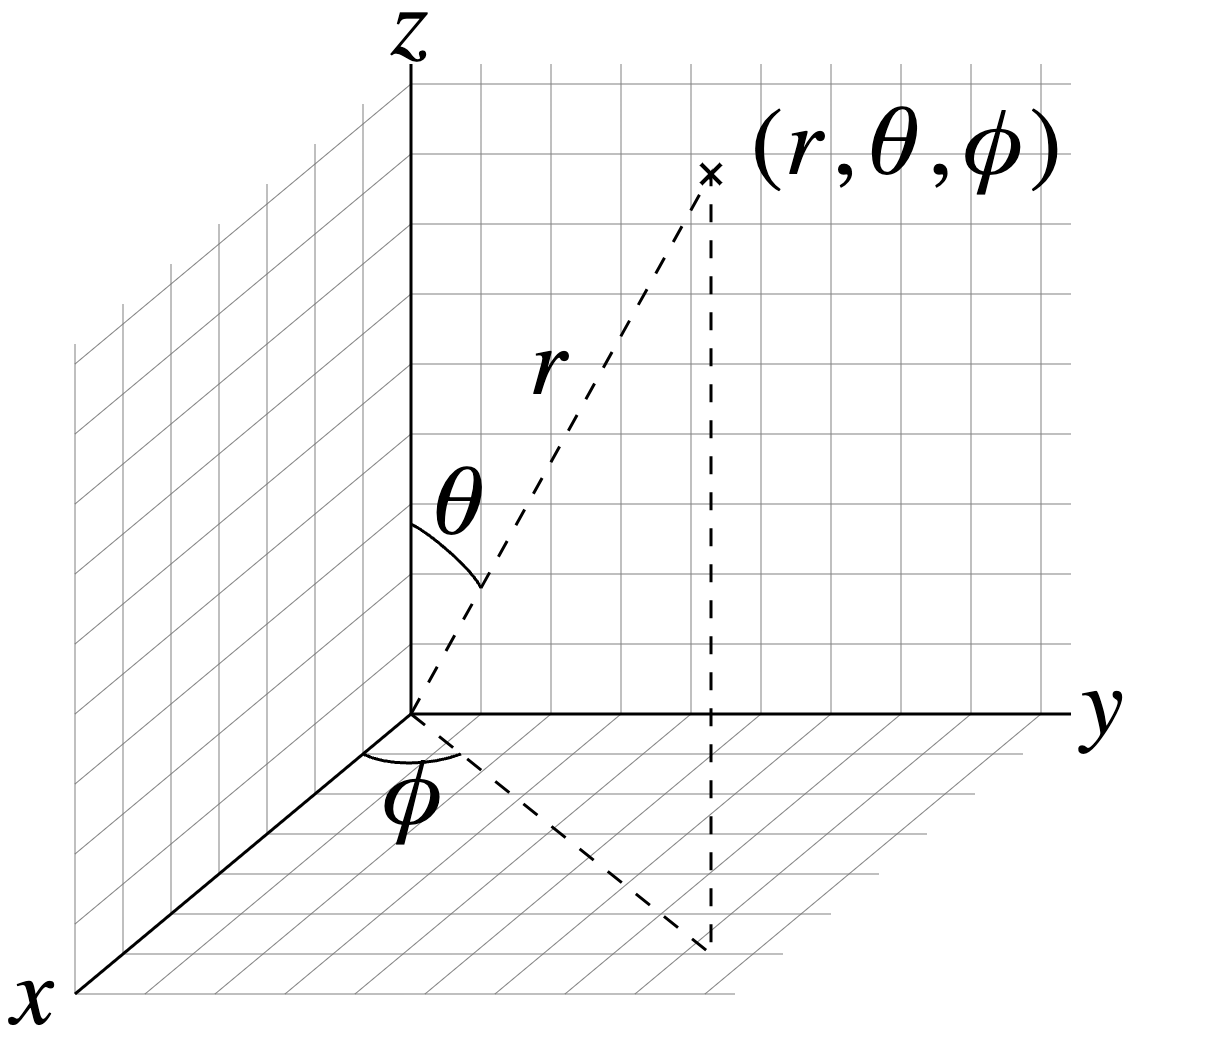
\includegraphics[width=5cm]{../../images/spherical_coords_wiki.png}
    \caption{Spherical coordinates from Wikipedia.}
    \label{fig:spherical_coordinates}
\end{figure}

\end{document}